\chapter{Tecniche di anonimizzazione}
Dato un dataset con informazioni personali sensibili vogliamo calcolare e rilasciare funzioni del dataset proteggendo la privacy individuale.\\

\noindent Gli attributi di un record di un dataset possono essere classificati in tre categorie:
\begin{itemize}
    \item \textbf{Identificatori espliciti}: permettono l'identificazione univoca dell'utente (es: nome, cognome, codice fiscale, ...)
    \item \textbf{Quasi-identificatori}: pezzi di informazioni che non sono di per sé identificatori univoci, ma sono sufficientemente ben correlati con un'entità da poter essere combinati con altri quasi-identificatori per creare un identificatore univoco (es: data di nascita, età, numero di telefono, ...);
    \item \textbf{Attributi sensitivi}: attributi che non dovrebbero essere collegabili all'utente e dipendono dal contesto (es: salario, malattie, ... ).
\end{itemize}

\noindent Un esempio di attributi è riportato in figura \ref{fig:14-1}.

\begin{figure}
    \centering
    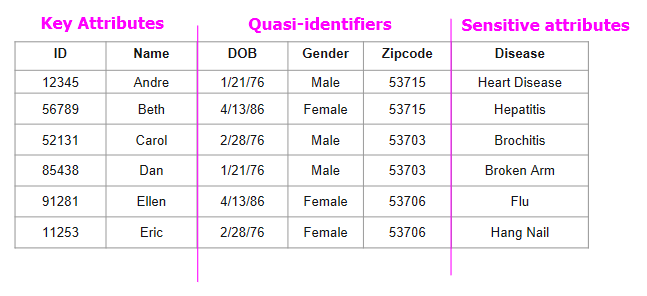
\includegraphics[width=0.8\textwidth]{images/14-1.png}
    \caption{Esempio di attributi}
    \label{fig:14-1}
\end{figure}

\section{Tecniche di per proteggere gli identificatori espliciti}
Esistono due tecniche per proteggere gli identificatori espliciti:
\begin{itemize}
    \item \textbf{Tokenization}: genera un token univoco per il dato;
    \item \textbf{Sostituzione}: sostituisce il valore di un attributo con un valore alternativo (scelto casualmente).
\end{itemize}

\noindent Queste tipo di tecniche non sono sufficienti a garantire la privacy degli utenti. 
\\

\noindent \underline{Esempio}
\\

\noindent Nel 2006 i ricercatori di AOL avevano preso tutte le query fatte dagli utenti in tre mesi e le avevano pubblicate in un dataset dopo aver applicato la tecnica di tokenization. Due giornalisti, analizzando il dataset, sono riusciti a identificare risalire all'idenittà di uno degli utenti le cui query erano state inserite nel dataset.
\\

\noindent Un altro attacco a cui queste tecniche sono vulnerabili è il \textbf{record linkage}: dato un dataset anonimizzato (dataset medico), a cui sono stati rimossi gli attributo identificatori, e uno pubblico (dataset cittadini votanti), incrociando gli attributi quasi-identificatori è possibile risalire all'identità della persona.

\section{K-Anonimity}
Introdotto per proteggersi dal record linkage. Prevede che:
\begin{itemize}
    \item Un record sia indistinguibile da almeno k-1 altri record per quanto riguarda i quasi-identificatori;
    \item Ogni classe di equivalenza contenga almeno k record che hanno gli stessi valori per i quasi identificatori.
\end{itemize}

\noindent Un esempio è riportato in figura \ref{fig:14-2}. uno dei problemi di questa soluzione è che se l'attaccante sa che Bob si trova nella prima classe di equivalenza (prime tre righe), allora ha $1/3$ di probabilità di indovinare.

\begin{figure}
    \centering
    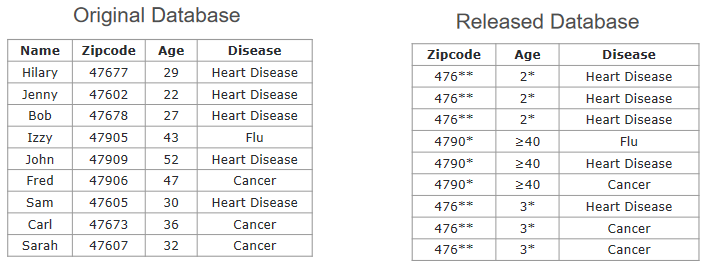
\includegraphics[width=0.8\textwidth]{images/14-2.png}
    \caption{Nel dataset rilasciato è stato rimosso il nome (identificatore); le prime 3 righe sono una classe di equivalenza.}
    \label{fig:14-2}
\end{figure}

\noindent Per raggiungere la K-Anonimity si usa la \textbf{generalizzazione}: si sostituiscono i quasi-identificatori con valori meno specifici finché non si ottengono K valori identici (partiziona i domini con valori ordinati in intervalli). Quando un attributo è troppo specifico o la generalizzazione non lo generalizza abbastanza, lo rimuovo (\textbf{soppressione} - comune con valori anomali). 

Esistono molti algoritmi nella letteratura che mirano a realizzare un'anonimizzazione "utile", ma spesso di solito senza alcuna chiara nozione di utilità.
\\

\noindent Esempi di K-anonimity: 
\begin{itemize}
    \item Applichiamo una formula che ritorna tre possibili valori di età: $>20$, $20<x\le30$, $30<x\le40$, $\ge40$ (\ref{});
    \item Raccogliamo sotto Grad School i valori Bachelor e Master.
\end{itemize}

\begin{figure}
    \centering
    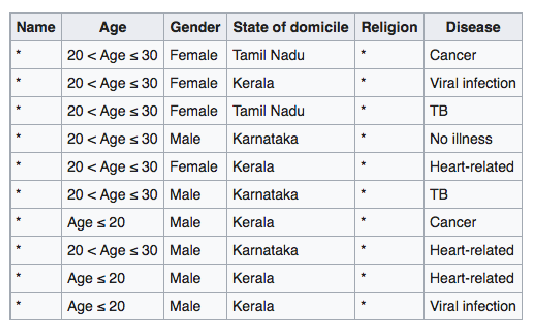
\includegraphics[width=0.6\textwidth]{images/14-3.png}
    \caption{L'attributo religione non serve nell'analisi e quindi lo rimuoviamo.}
    \label{fig:14-3}
\end{figure}

\noindent La K-Anonimity non fornisce privacy nel caso in cui valori sensibili nella stessa classe di equivalenza mancano di diversità oppure l'attaccante ha conoscenze di background (\ref{fig:14-4}) 

\begin{figure}
    \centering
    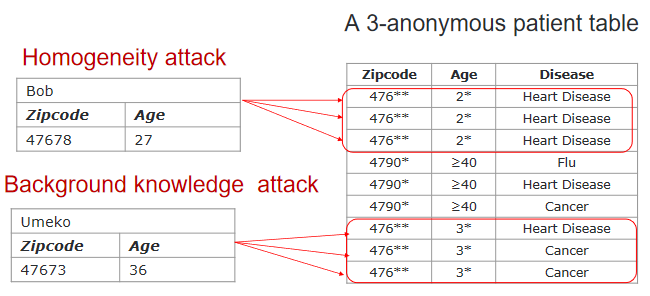
\includegraphics[width=0.8\textwidth]{images/14-4.png}
    \caption{Se l'attaccante è vicino di casa di Boc e conosce il suo zip code ed età, può scoprire che soffre di heart desease, in quanto nella classe di equivalenza di Bob, tutti soffrono di quella malattia. Sapendo che Umineko è giapponese e i giapponesi difficilmente soffrono di problemi al cuore, è molto probabile che abbia in cancro.}
    \label{fig:14-4}
\end{figure}

\section{L-diversiry}
Introdotto per risolvere i problema della K-Anonimity. Prevede che attributi sensibili nella stessa classe di equivalenza di quasi-identificatori abbiano valori diversi (\ref{fig:14-5}). Nello specifico:
\begin{itemize}
    \item Ogni classe di equivalenza deve avere almeno I valori sensibili ben rappresentati;
    \item Non previene attacchi di inferenza probabilistica.
\end{itemize}

\begin{figure}
    \centering
    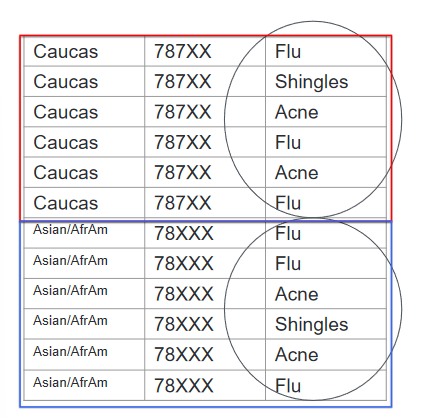
\includegraphics[width=0.4\textwidth]{images/14-5.png}
    \caption{Esempio.}
    \label{fig:14-5}
\end{figure}

\begin{definition}[Entropia l-diversità]
    Ogni classe di equivalenza non solo deve avere valori sensibili abbastanza diversi, ma
    anche i diversi valori sensibili devono essere distribuiti in maniera sufficientemente omogenea. L'entropia della distribuzione dei valori sensibili in ogni classe di equivalenza deve essere almeno $\log(l)$.

    \noindent L'entropia di una classe di equivalenza $E$ è definita come:
    \begin{align*}
        Entropy(E) = - \sum_{s \in S} p(E, s) \log{p(E, s)}
    \end{align*}

    \noindent dove $S$ è il dominio dell'attributo sensibile e $p(E, s)$ è la frazione di record in $E$ che ha valore sensibile $s$.
\end{definition}

\noindent Questa tecnica è debole al \textbf{sensitive attribute disclosure} (\ref{fig:14-6}).

\begin{figure}
    \centering
    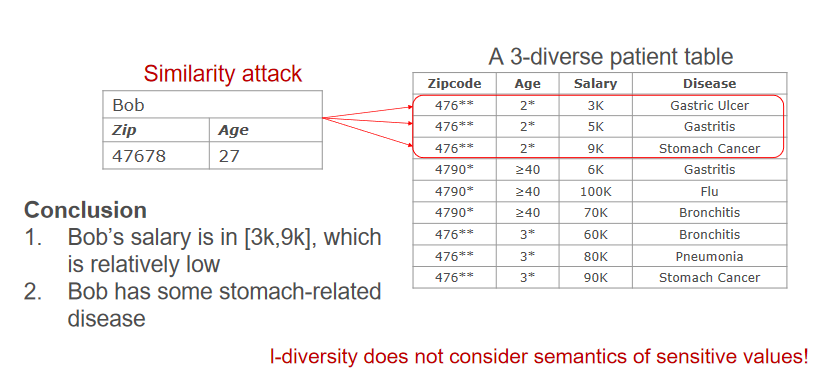
\includegraphics[width=0.9\textwidth]{images/14-6.png}
    \caption{Esempio di sensitive attribute disclosure.}
    \label{fig:14-6}
\end{figure}

\noindent La L-diversity soffre di altri vulnerabilità:
\begin{itemize}
    \item Se l'attaccante sa che 50\% del dataset è HIV+ e il restante 50\% è HIV-, può dire che Bob è al 50\% HIV+ (viola privacy);
    \item Se 49 record sono HIV+ e 1 è HIV-, allora molto probabilmente Bob è HIV+ (problema distribuzione valori).
\end{itemize}

\noindent In generale, L-diversity non considera la semantica e la distribuzione dei valori sentitivi.

\section{T-closeness}

Prevede che la distribuzione degli attributi sensibili all'interno di ciascun gruppo di quasi-identificatori sia "vicina" alla loro distribuzione nell'intero database originale ().

\begin{figure}
    \centering
    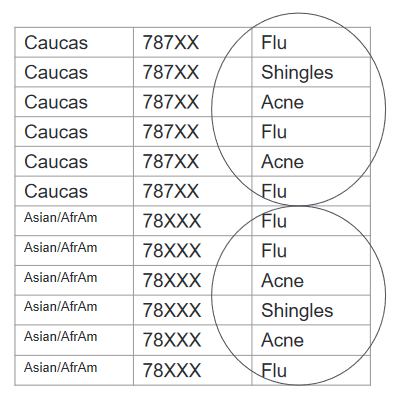
\includegraphics[width=0.4\textwidth]{images/14-7.png}
    \caption{Esempio di T-closeness.}
    \label{fig:14-7}
\end{figure}

\noindent In generale, semplicemente anonimizzare i dati non è sicuro: i dati presumibilmente anonimizzati spesso contengono modi alternativi di identificazione (quasi identificatori). L'accesso alle informazioni ausiliarie appropriate può quindi comportare la reidentificazione.

\section{Differential privacy}
Supponiamo di avere un dataset nel quale consentiamo solo analisi statistiche, quindi solo query che ritornano valori aggregati. Questo tipo di analisi è sicura? In teoria si, ma nella pratica no. 

\begin{figure}
    \centering
    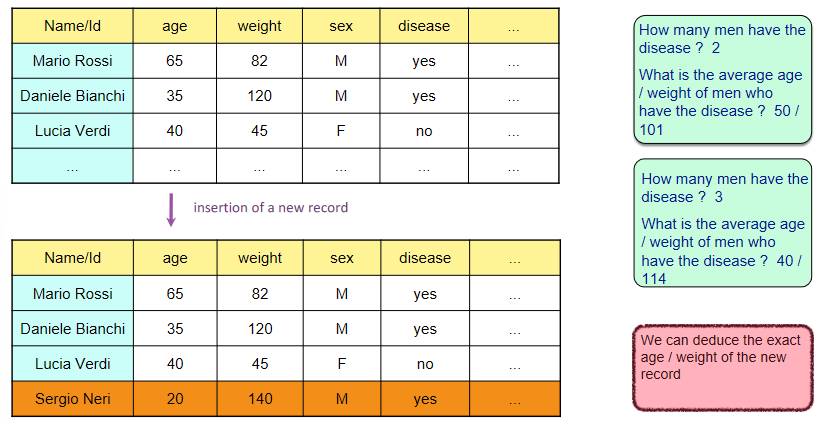
\includegraphics[width=0.8\textwidth]{images/14-8.png}
    \caption{Esempio di Reconstruction Attack.}
    \label{fig:14-8}
\end{figure}

\noindent Supponiamo di sapere che nel dataset originale 2 uomini abbiano il diabete e che età e peso medi degli uomini con diabete siano 50 anni e 101 kg. Rieseguendo le due query dopo l'aggiunta del nuovo record, scopriamo che i malati sono saliti a 3 e che età e peso medi sono cambiati. Possiamo quindi ricostruire età e peso esatti per il nuovo record, oltre a sapere che soffre di diabete.

Quindi la restrizione alle query aggregate non è sufficiente: anche queste query potrebbero trapelare informazioni sugli individui (\textbf{Reconstruction Attack}).
\\

\noindent Da questo è stato introdotto il concetto di \textbf{differential privacy}: qualsiasi rischio relativo alle informazioni per una persona non dovrebbe cambiare in modo significativo a seguito dell'inclusione o meno delle informazioni di quella persona nell'analisi. In generale vogliamo che la differenza tra i risultati delle due analisi sia un valore trascurabile $\varepsilon$.
\\

\noindent La differential privacy garantisce due proprietà:
\begin{enumerate}
    \item \textbf{Post processing invariance}: il rischio non aumenta se i dati non vengono toccati ancora;
    \item \textbf{Robustness under Composition}: se eseguiamo una serie di analisi sul dataset che soddisfano la privacy differenziale, ciascuna col proprio $\varepsilon$, l'applicazione di queste analisi in sequenza genera un $\varepsilon$ totale pari alla somma delle singole $\varepsilon$.
\end{enumerate}

\section{Implementazione privacy differenziale}
Uno dei metodi più usati è il Global Sensitivity Method, che usa la distribuzione di Laplace. Noi vogliamo effettuare un'analisi sul dataset. Il metodo dice di prendere il valore della funzione e di aggiungerci del rumore, preso da una variabile che ha una distribuzione secondo quella di Laplace, e ritorniamo il risultato.

Supponiamo che la nostra funzione calcoli la media dei valori sensitivi. Per prima cosa calcoliamo la global sensitivity della funzione, ottenuta dalla differenza tra la funzione applicata al dataset D che stiamo considerando e la funzione applicata al dataset D' che differisce dal primo per al più un record (calcoliamo la differenza record per record, e ritorniamo quella con il valore assoluto maggiore). Ottenuta la global sensitivity aggiungiamo il rumore Z, data da:
\begin{align*}
    Z = \frac{global\_sensitivity}{\varepsilon} \cdot distribuzione\_Laplace(0, 1)
\end{align*}

\noindent In generale, la privacy differenziale può essere usata in:
\begin{itemize}
    \item Analisi statistiche (conteggi, media, mediana, ...);
    \item Machine learning supervisionato e non supervisionato (classificazione, regressione, ...);
    \item Generazione di dati sintetici.
\end{itemize}

\paragraph{US census bureau 2020} In america c’è un censimento periodico, e si possono fare query su questi dati. L’analisi soddisfa la privacy.
\paragraph{Google} Ha un’implementazione open source che si chiama RAPPOR, ed è usata per fare analisi sulle ricerche degli utenti.
\paragraph{Apple} Non ha reso pubblico l’algoritmo. Alcuni ricercatori vi hanno avuto l’accesso e hanno fatto reverse engineering del codice, e non è così private perché usa un epsilon
intorno a 11.
\paragraph{Privacy differenziale locale} Sia google che apple usano la privacy differenziale locale per avere info su dati telemetrici; anziché catturare il dato reale, aggiungono al dato singolo un rumore, e questo dato perturbato può comunque essere analizzato. Apple lo usa per mantenere traccia di quali sono le emoji più usate.
\paragraph{Implementazioni della privacy differenziale }Ci sono due implementazioni della privacy differenziale: Tensor flow (google) e Opacus (facebook).












